\documentclass[a4paper,9pt,russian]{article}
\usepackage{cmap}
\usepackage{pgfplots}
\usepackage{hyperref}
\usepackage[T2A]{fontenc}
\usepackage[utf8]{inputenc}
\usepackage[russian]{babel}
\usepackage{graphicx}
\usepackage{xcolor}
\usepackage{amssymb}
\usepackage{amsmath}
\usepackage{physics}
\usepackage{mathrsfs}
\usepackage{amsfonts}
\usepackage{cancel}

\newcommand{\I}{\mathscr{I}}
\renewcommand{\-}{\bar}
\newcommand{\T}{\theta}
\newcommand{\D}{\delta}
\newcommand{\K}{\varkappa}

\title{РГР 1}
\author{А. В. Козлов} 
\begin{document}
\maketitle
\begin{abstract}

\end{abstract}
\section{Формулировка задачи}
Дано двумерное отображение:
\begin{equation}\label{->}
\begin{cases}
	\- \I = \I + k \sin{\T}\\
	\- \T = \T + \dfrac{1}{\- \I}
\end{cases}
.
\end{equation}
\[
" x " t "
.\]  
Необходимо определить условие возникновения хаоса двумя способами: через критерий Чирикова и через критерий многопотоковости. Так же требуется воспользоваться приближением Фокера--Планка, получить с его помощью одноимённое уравнение и определить его стационарное решение.
\section{Критерий многопотоковости}
Перепишем отображение (\ref{->}) в более приятном виде:
\begin{equation}\label{->2}
\begin{cases}
	\- \I  = \I + k \sin{\T}\\
	\- \T = \T + \dfrac{1}{\I + k \sin{\T}}
\end{cases}
.
\end{equation}
Критерий возникнавения глобального хаоса выглядит следующим образом:
\begin{equation}\label{mu}
	\eval{\dv{\- \I}{\- \T}}_{\I}=\infty.
\end{equation}
Для рассматриваемого отображения критерий принимает следующий вид:
\[
	\dv{\- \I}{\- \T} = \dfrac{\pdv{\- \I}{\T}}{\pdv{\- \T}{\T}} = \dfrac{k \cos{\T}}{1 - \dfrac{k \cos{\T}}{\qty(\I + k \sin{\T})^2}} = 
	\dfrac{k \cos{\T}\qty(\I +k \sin{\T})^2}{\qty(\I + k \sin{\T})^2-k \cos{\T}}=\infty
.\] 
Откуда следует уравнение:
\begin{equation}\label{0}
	\qty(\I + k \sin{\T})^2 = k \cos{\T},
\end{equation}
для которого нужно найти область параметров, внутри которой существуют решения данного уравнения. Для удобства анализа перепишем (\ref{0}) в более удобный вид:
\begin{equation}\label{1}
	\I + k \sin{\T} = \sqrt{k \sin{\T}}
\end{equation}
Рассмотрим предельный случай при $k \ll 1$. Графически это можно представить следующим образом.
\begin{figure}[h]
 \centering
 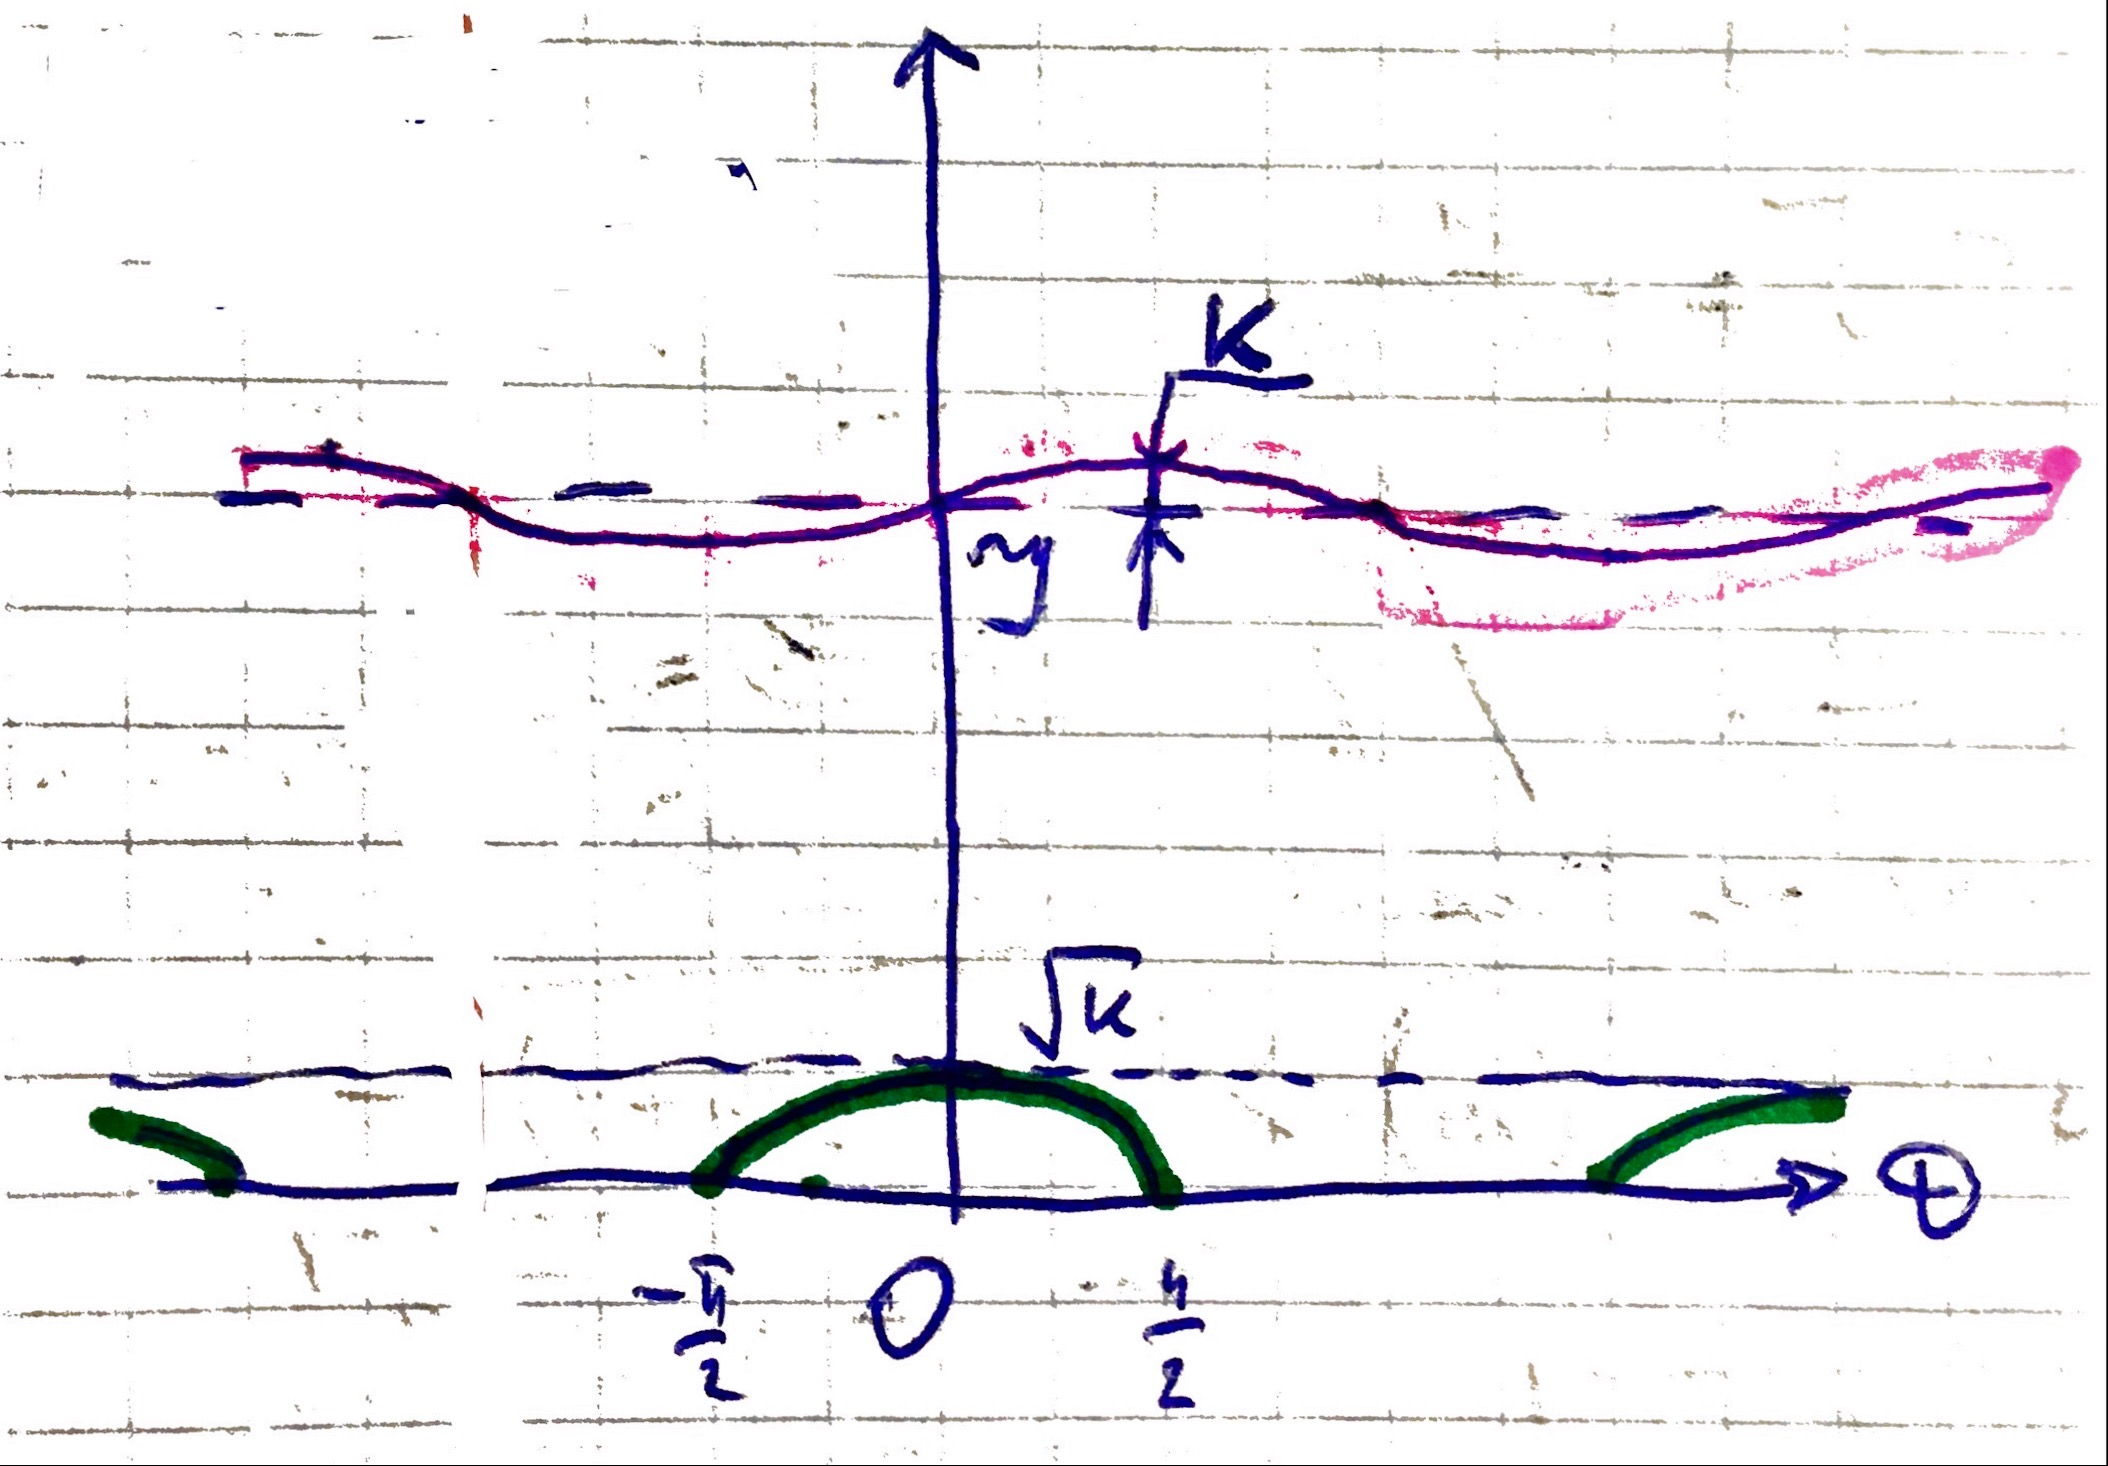
\includegraphics[width = 80mm]{graf/graf1.JPG}
 \caption{График левой и правой части уравнения (\ref{1}) при $k \ll 1$}
 \label{graf}
\end{figure}
\par
Из графического представления видно, что для того, чтобы пересечение (а, следовательно, и решение) существовало, нужно потребовать в нулевом приближении $\I \le \sqrt{k}$. Это достаточно грубое условие, оно отражает то, что осциллирующая около $\I$ функция заденет корень косинуса.
\par
Теперь обратим свой взор на другой предельный случай: $k \gg 1$. Опять изобразим его графически.
\begin{figure}[h]
 \centering
 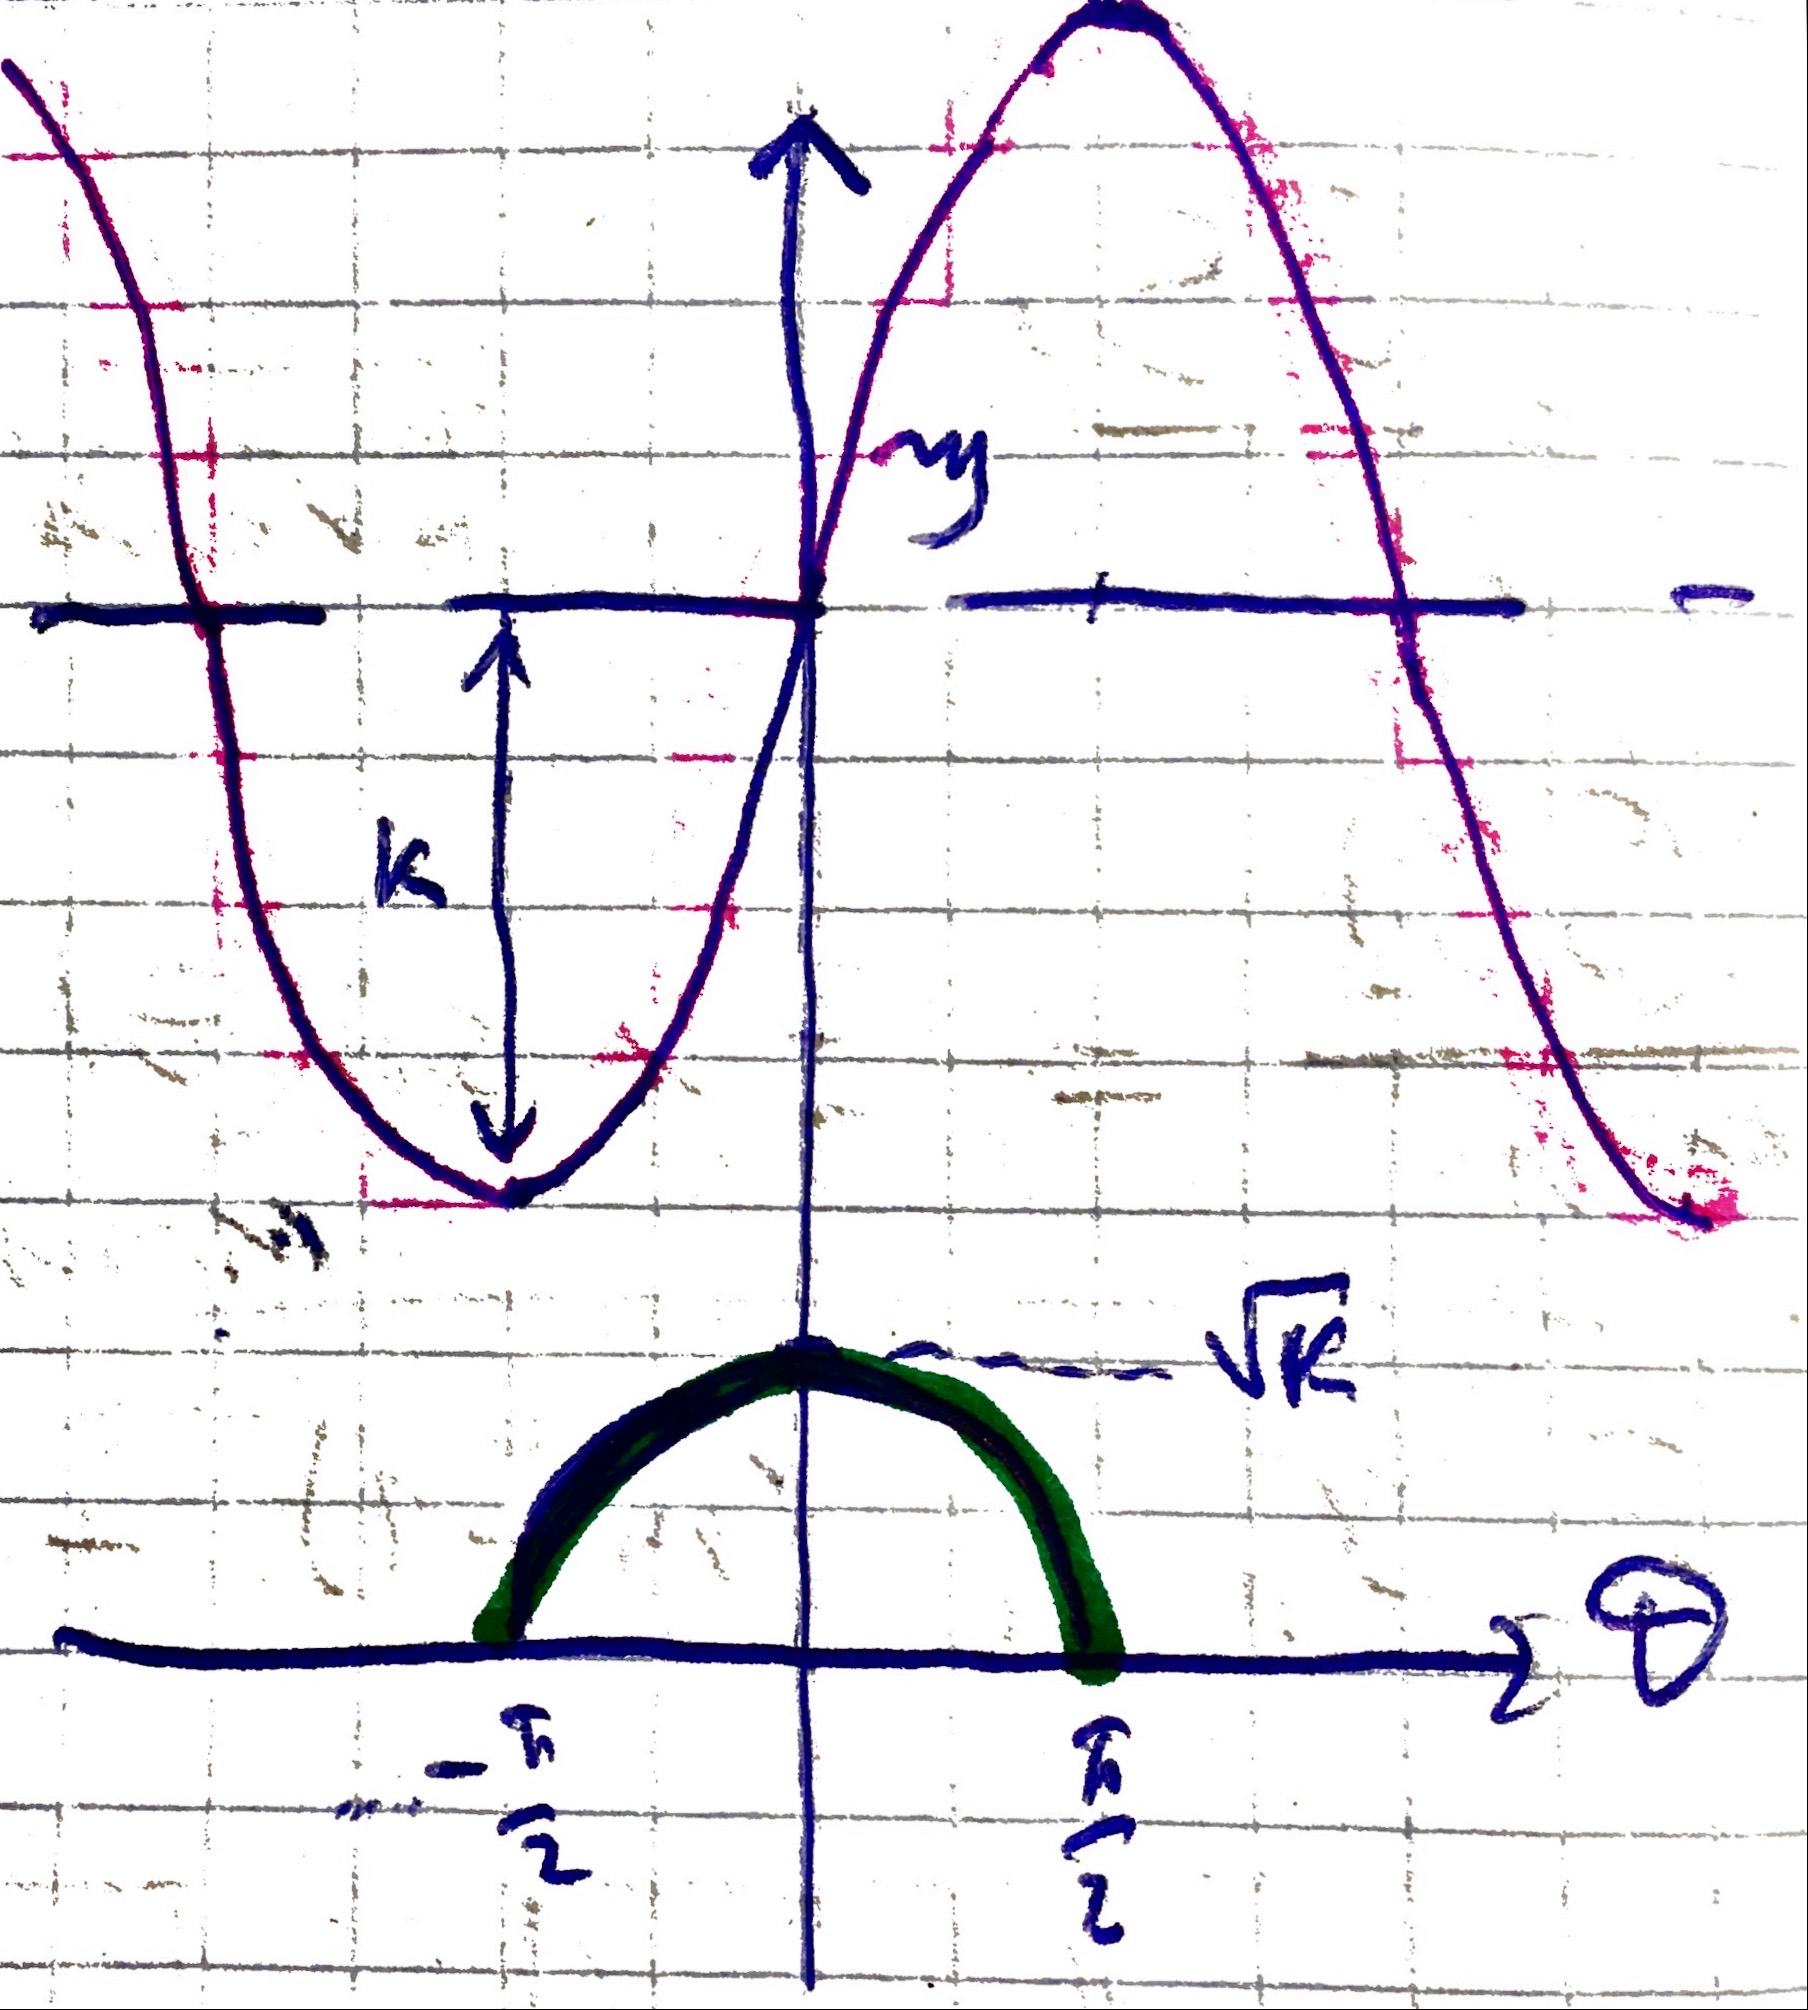
\includegraphics[width = 70 mm]{graf/graf2.JPG}
 \caption{График левой и правой части уравнения (\ref{1}) при $k \gg 1$}
 \label{graf}
\end{figure}
\par
Видно, что для наличия решения нужно требовать опять--таки в нулевом приближении $\I \le k$. Тогда получаем такой график $k \qty(\I)$ (см.\ref{graf3} ).
\begin{figure}
 \centering
 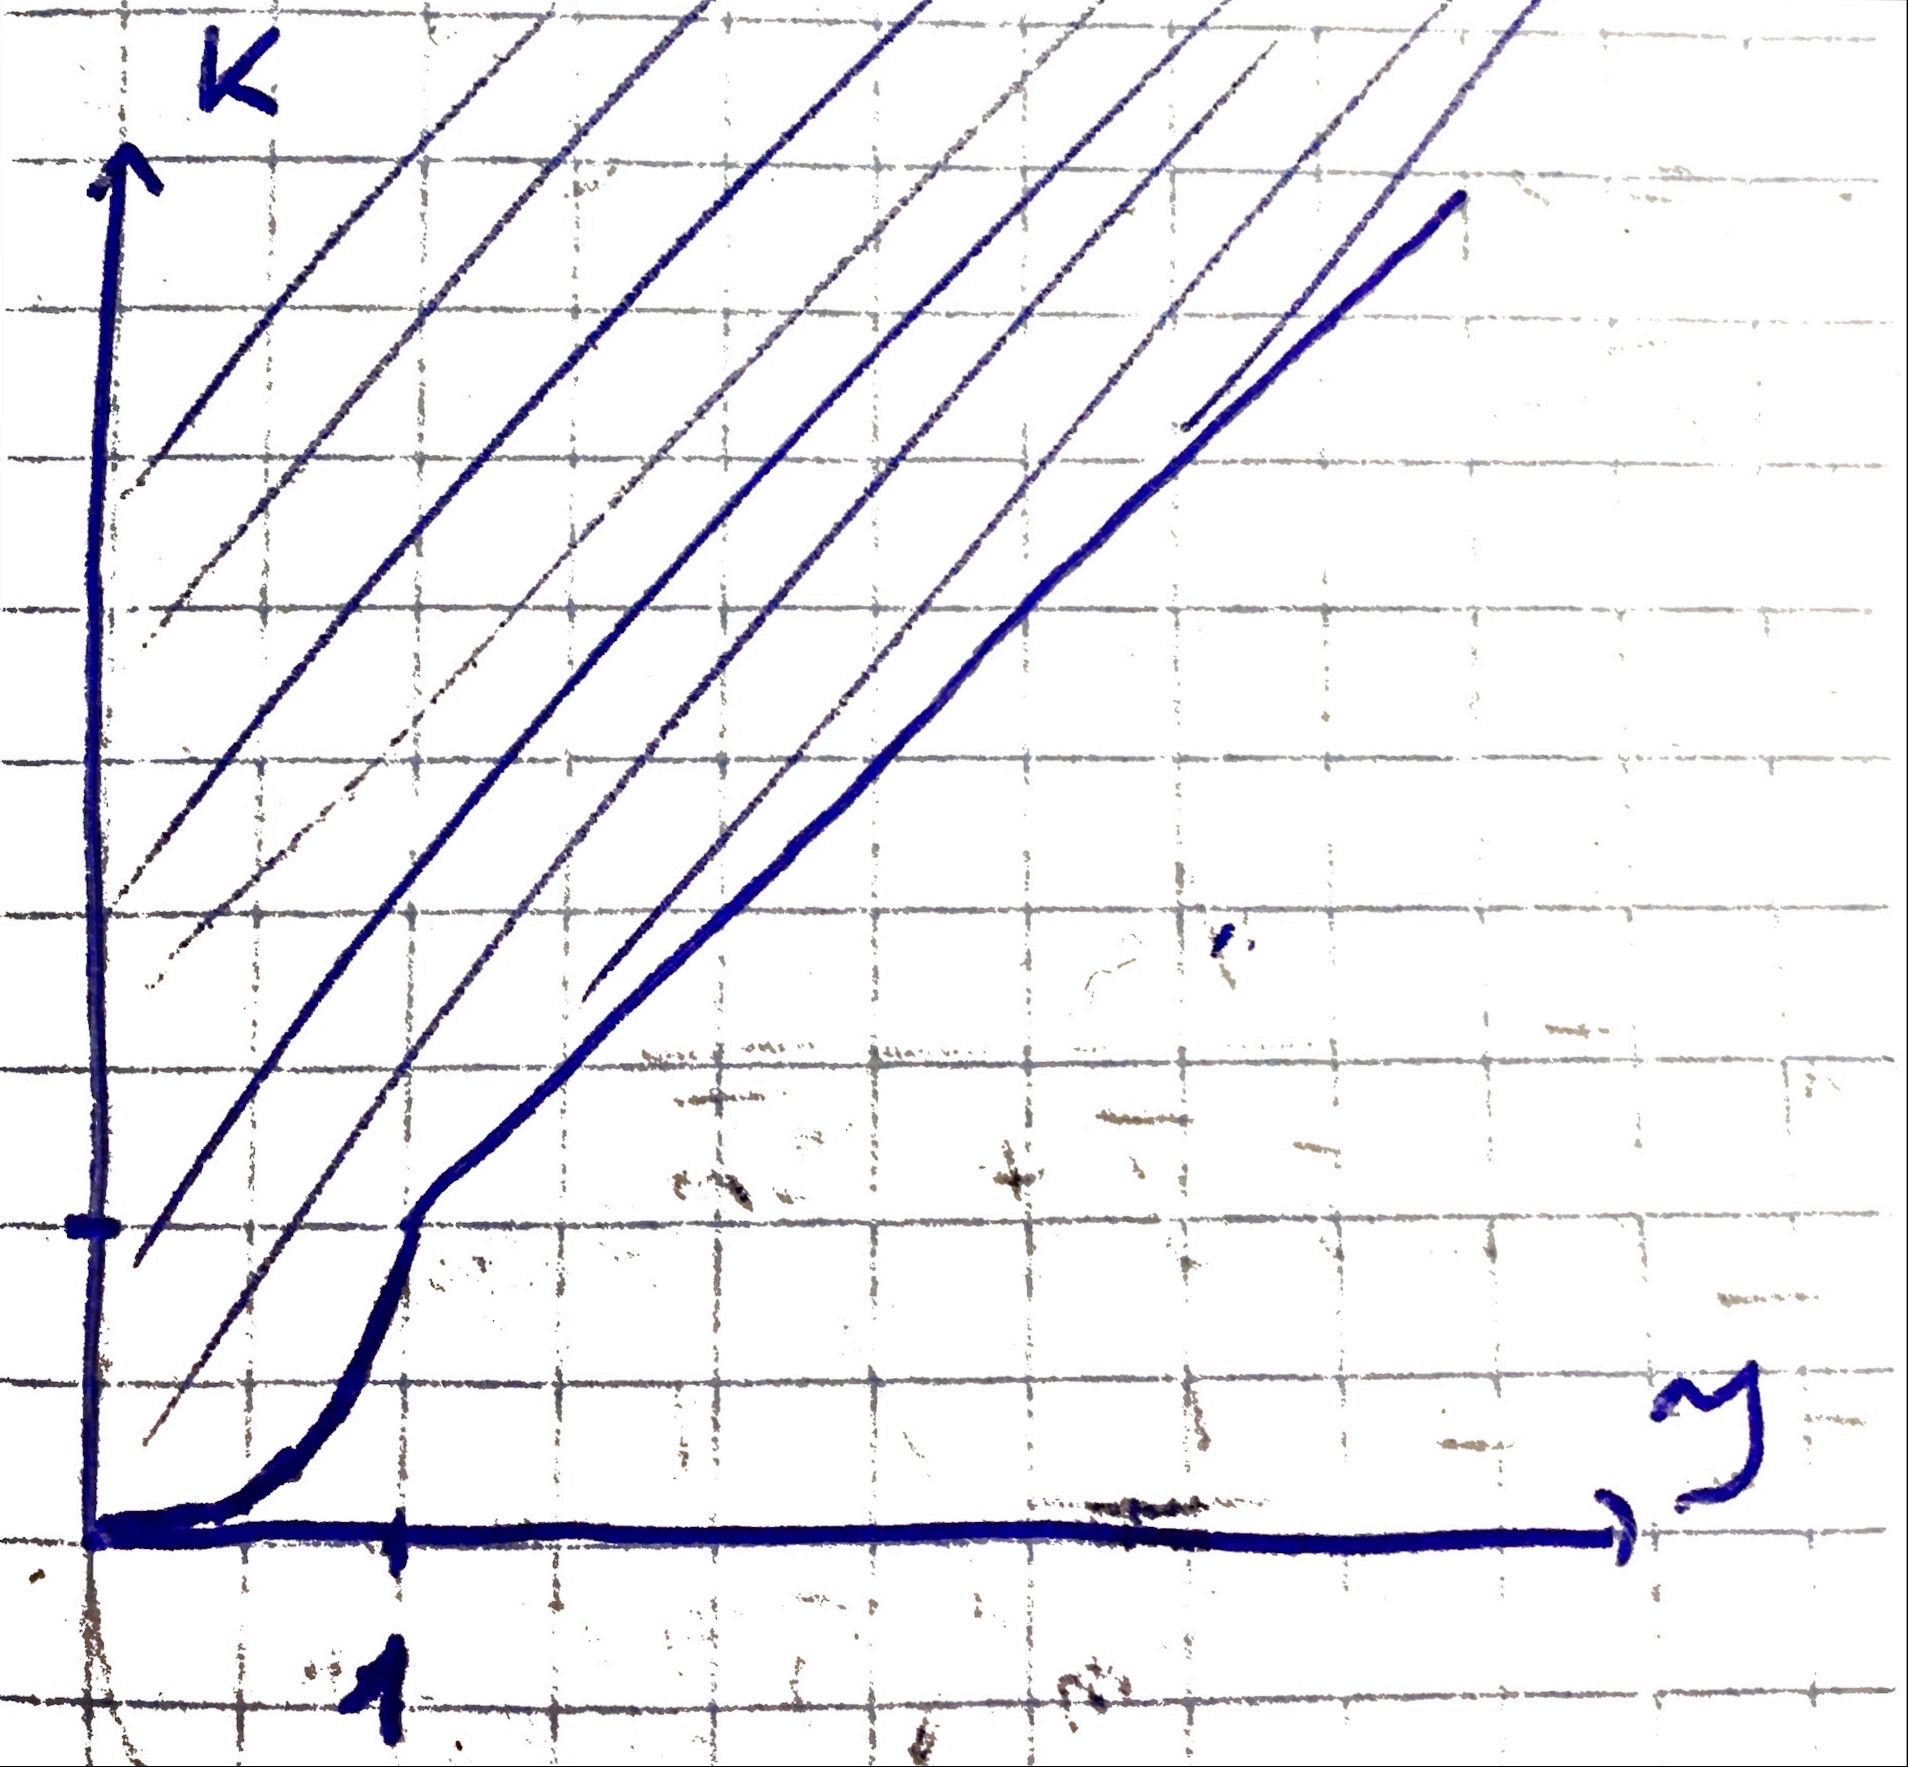
\includegraphics[width = 70mm]{graf/graf3.JPG}
 \caption{Область, где возникает глобальный хаос согласно методу многопотокости}
 \label{graf3}
\end{figure}
\section{Критерий перекрытия резонансов}
Напомню, что рассматриваем мы данное отображение:
\begin{equation}\label{->3}
\begin{cases}
	\- \I = \I + k \sin{\T}\\
	\- \T = \T + \dfrac{1}{\I - k \sin{\T}}
\end{cases}
.
\end{equation}
Так как $\sin{\T}$ периодичен с периодом  $2 \pi$, то и само отображение будет периодичным по  $\T$ с периодом  $2\pi$.
\par
Найдём стационарные точки:
\begin{equation}\label{st}
\begin{cases}
	k \sin{\T} = 0\\
	\dfrac{1}{\I}=2 \pi m, \quad m \in \mathbb{Z} 
\end{cases}
,
\end{equation}
где второе уравнение следует из следующих рассуждений. Угол $\T$ кратен  $\pi$ (из первого уравнения системы), а само отображение периодично по $\T$ с периодом  $2\pi$, то есть, выходит, что при применении отображения угол стационарного состояния может сместиться на целое число $2\pi$. 
\par
Тогда имеем следующие стационарные состояния (сетка стационарных состояний):
\begin{equation}\label{sta}
\begin{cases}
	{\T}_n = \pi n\\
	{\I}_m=\dfrac{1}{2 \pi m}, \quad m \in \mathbb{Z} 
\end{cases}
.
\end{equation}
Исследуем систему вблизи стационарного состояния. Для этого введём обозначения:
\begin{align}\label{del}
&\D \T = \T - \T_n;  \\
&\D \I = \I - \I_m. 
\end{align}
И полагаем $\abs{\D \T},\abs{\D \I} \ll 1$. Теперь переходим куравнениям в непрерывном времени от уравнений в дискретном времени. Первое уравнение отображения (\ref{->}):
\begin{align}
 &\- \I = \I + k \sin{\T};\\
 &\D \- \I = k \sin \qty{\D \T + \T_n} + \D \I;\\
 & \pdv{\qty(\D \I)}{n} = k \qty(\sin{\D \T}\cos{\T_n}+\sin{\T_n}\cos{\D \T}) =\qty{\T_n = \pi n}= \pm  k \sin{\D \T};\\
 & \pdv{\qty(\D \I)}{n} = \pm  k \sin{\D \T}.
\end{align}
Второе уравнение отображения (\ref{->}):
\begin{align}
 &\- \T = \T + \dfrac{1}{\- \I};\\
 &\D \- \T + \- \T_n = \D \T + \T_n + \dfrac{1}{\D \- \I + \- \I_m};\\
 &\pdv{\qty(\D \T)}{n}= -\qty(\T - \- \T) + \dfrac{1}{\I_m}\qty(\dfrac{1}{1 + \frac{\D \I}{\I_m}});\\
 &\pdv{\qty(\D \T)}{n}\approx \xcancel{-\qty(\T - \- \T)} +\xcancel{\dfrac{1}{\I_m}} - \dfrac{\D \I}{\I_m^2};\\
 &\pdv{\qty(\D \T)}{n} = -\qty(2\pi m)^2 \D \I.
\end{align}
Тогда получаем систему нелинейных уравнений:
\begin{equation}\label{syst}
\begin{cases}
	\pdv{\qty(\D \I)}{n} = \pm  k \sin{\D \T}\\
\pdv{\qty(\D \T)}{n} = -\qty(2\pi m)^2 \D \I
\end{cases}
.
\end{equation}
Интеграл энергии для неё будет иметь вид: $$H = \dfrac{\qty(2\pi m)^2\qty(\D \I)^2}2  \mp k \cos{\D \T}.$$
Если на сепаратрисе энергия равна $k$ (а она этому и равна на сепаратрисе, то есть это максимальное значение энергии при нулевом $\D \I$), то тогда можно найти амплитуду сепаратрисы:
 \[
\dfrac{\qty(2\pi m)^2\qty(\D \I)^2}2  - k = k
,\]
\[
\D \I_{max} = \dfrac{\sqrt k}{\pi m}
.\]
Критерий Чирикова заключается в том, что если сепаратрисы пересекаются, то возникает глобальный хаос. Поэтому пишем условие, что сумма ампилитуд двух соседних сепаратрис больше расстояния между их средними значениями:
\[
	\dfrac{\sqrt k}{\pi \qty(m+1)} +\dfrac{\sqrt k}{\pi m}\ge \dfrac{1}{2 \pi m} - \dfrac{1}{2 \pi \qty(m+1)} 
.\]
Рассматривая предельный случай $m\rightarrow \infty$, получается оценка:
\[
	2\dfrac{\sqrt k}{\pi m} \ge \dfrac{1}{2 \pi m}\qty(1-\dfrac{1}{1+\dfrac{1}{m}})
,\] 
---расскладваем правую часть в ряд Тейлора до первого порядка---
\[
	\dfrac{\sqrt k}{\pi m} \ge \dfrac{1}{4 \pi m}\vdot 
	\dfrac{1}{m}
,\] 
\[
k \ge \dfrac{1}{16m^2}
.\]
Откуда видно, что получается более грубая оценка, чем при работе с критерием многопотоковости.
\section{Приближение Фокера--Планка}
Рассматриваем отображение (\ref{->3}). При сильном хаосе согласно приближению Фокера--Планка распределение частиц по $\T$ однородно. Это значит, что если обозначить за $\Phi\qty(\I,\T)$ истиную функцию распределения, то:
\begin{equation}\label{den}
	\Phi\qty(\I,\T) \approx \frac{1}{2\pi} F\qty(\I)
	,\text{ где } F\qty(\I) = \int \Phi\qty(\I, \T) \dd \T.
\end{equation}
\par
За один шаг отображения полная функция распределения будет:
\begin{equation}\label{in_1}
	\- \Phi\qty(\I, \T)=\Phi\qty(\tilde \I, \tilde \T)=\Phi\qty(\I - k \sin{\T}, \T - \dfrac{1}{\I}),
\end{equation}
где $\tilde \I, \tilde \T$ задаются как переменные, предшествующие переменным $\I, \T$: 
\[
\begin{cases}
	\I = \tilde \I + k \sin{\tilde \T}\\
	\T = \tilde \T + \dfrac{1}{\I}
\end{cases}
.\]
Если вернуться к (\ref{in_1}), то можно продолжить равенство таким интегралом:
\begin{equation}\label{in_2}
	\- \Phi\qty(\I,\T) = \int \D\qty(\I - \I' - k\sin{\T'})\D\qty(\T - \dfrac{1}{\T' + k \sin{\T'}})\Phi\qty(\I',\T')\dd\I' \dd\T',
\end{equation}
куда подставляем аппроксимацию функции распределения из (\ref{den}) и интегрируем по $\T$:
\begin{align}\label{in_3}
	\int\- \Phi\qty(\I,\T)\dd{\T} &=\dfrac{1}{2\pi} \int \D\qty(\I - \I' - k\sin{\T'})\D\qty(\T - \frac{1}{\T' + k \sin{\T'}})\vdot \\
				      &\vdot F\qty(\I')\dd\I' \dd\T'\dd\T=\\ 
				      &=\int \dd\T' \dd\I' \D\qty(\I - \I' -k \sin{\T'})\frac{F\qty(\I')}{2\pi}.
\end{align}
Теперь пришло время воспользоваться медленностью $F\qty(\I')$ около $\I' = \I$. Разлагаем в ряд Тейлора:
 \[
	 F\qty(\I{'})=F\qty(\I)+\eval{\pdv{F}{\I{'}}}_\I \qty(\I{'} - \I) + \frac12\eval{\pdv[2]{F}{\I{'}}}_\I \qty(\I{'} - \I)^2+\ldots
 \] 
Аналогично лекционному материалу, замечаем, что первый порядок вносит нулевой вклад, второй же порядок не зануляется в интеграле и даёт:
\begin{equation}\label{in_4}
	\- F - F = \eval{\pdv[2]{F}{\I{'}}}_\I \dfrac{k^2}{4}.
\end{equation}
Заменяем левую часть на производную, получаем уравнение диффракции:
\begin{equation}\label{dif_eq}
	\pdv{F}{n}=\frac{k^2}{4}\eval{\pdv[2]{F}{\I{'}}}_\I.
\end{equation}
Используем преобразование Фурье $\tilde F\qty(\varkappa) = \int e^{i \I{'} \K} F\qty(\I{'}, n) \dd \I{'}$ к уравнению дифракции:
\[
\pdv{\tilde F}{n} = \dfrac{k^2}{4}\qty(-\K^2)\tilde F
.\]
Его решением будет: 
\[
	\tilde F\qty(\K, n) = \tilde F\qty(\K, 0) e^{-\K^2 n \frac{k^2}{4}}
.\]
Применим к нему обратное преобразование Фурье: $$F =\frac{1}{2\pi} \int \tilde F e^{-i\K\I{'}}\dd \K.$$
Тогда получаем общее решение дифракционного уравнения:
\begin{multline}
	F\qty(\I{'}, n) =\dfrac{1}{2\pi}\int \tilde F\qty(\K, 0) e^{-\K^2 n \frac{k^2}{4}}\dd\K =\\ = \dfrac{1}{2\pi}\int\qty{F\qty(\I, 0) e^{ik\I}\dd \I} e^{-\K^2 n \frac{k^2}{4}}\dd\K.
\end{multline}
\end{document}
